\chapter{Validación experimental}\label{resultados}

Este capítulo describe los experimentos realizados en los entrenamientos con distintas configuraciones de parámetros combinando el número de acciones, el número de puntos de percepción y los circuitos. De estos experimentos se obtienen resultados que indican la mejor combinación para cada conjunto de prueba así como la mejor configuración global que resuelve la conducción autónoma y han permitido extraer varias lecciones sobre aplicar aprendizaje por refuerzo al contexto robótico.\\

%%%%%%%%%%%%%%%%%%%%%%%%%%%%%%%%%%%%%%%%%%%%%%%%%%%%%%%%%%%%%%%%%%%%%%%%%%%%%%%%%%%%%%%%%%%%%%%%%%%%%%%%%%%%%%%%
\section{Parámetros generales del aprendizaje}\label{parametros-generales}

En esta sección se describen las características generales de los entrenamientos por refuerzo y define los diferentes escenarios donde se realizan esos entrenamientos y donde se evalúan los `cerebros' obtenidos con el aprendizaje por refuerzo.\\

A nivel general todos los entrenamientos tienen una \textit{duración de 2 horas}. Se define este valor debido a la complejidad creciente que existe cuando se aumentan el número de percepciones (1, 2 y 3) y el número de acciones (3, 5 y 7). La combinación más alta de posibilidades, 3 niveles de percepción con 7 acciones posibles, necesita mayor tiempo de entrenamiento dado que requiere de un mayor tiempo de exploración del espacio de estados. Este valor permite un equilibrio entre convergencia y tiempo razonable de entrenamiento y permite comprar de un modo justo todas las combinaciones de aprendizaje, pues a todas ellas se les concede el mismo tiempo de entrenamiento.\\

Para todos los entrenamientos se fijan los parámetros globales que definen el algoritmo de aprendizaje por refuerzo Q-Learning (\textit{alpha}, \textit{gamma} y \textit{epsilon}). Los valores de estos parámetros se han ajustado a través de diferentes entrenamientos hasta conseguir unos valores que equilibran el aprendizaje con la resolución del ejercicio. Estos valores son:\\

\begin{itemize}
    \item \textbf{$\alpha$}: 0.8. Este valor es elegido por los buenos resultados que retorna el algoritmo en cuanto a número de episodios, tamaño de la Tabla-Q y tiempo de entrenamiento si se compara con el valor original ($0.2$).
    \item \textbf{$\gamma$}: 0.9. Fijado por la librería inicialmente así como por diferente bibliografía~\cite{oreily} ~\cite{pytorch_drl}.
    \item \textbf{$\epsilon$}: 0.99. Con un valor alto inicialmente, en cada episodio se le aplica un factor de descuento de $0.998$ que hará que el parámetro $\epsilon$ disminuya paulatinamente hasta el final del entrenamiento.\\
\end{itemize} 

Los entrenamientos se realizan en dos de los tres circuitos creados: en el circuito Simple y en el circuito de Nürburgring, dejando el circuito de Montreal únicamente para las evaluaciones. En ambos circuitos se realizan los entrenamientos con todas las combinaciones posibles entre los diferentes niveles de percepciones y varios conjuntos de acciones repitiéndose el experimento 3 veces para cada combinación con el objetivo de obtener una media más fiable que hace más representativo el resultado.\\

Tanto los entrenamientos como las posteriores evaluaciones ha sido realizadas con un ordenador portátil MSI gs63 con un procesador Intel i7 de 7ª generación, 16 Gb de memoria RAM y un disco duro SSD M.2 de 256 Gb.\\

%%%%%%%%%%%%%%%%%%%%%%%%%%%%%%%%%%%%%%%%%%%%%%%%%%%%%%%%%%%%%%%%%%%%%%%%%%%%%%%%%%%%%%%%%%%%%%%%%%%%%%%%%%%%%%%%
\section{Análisis de entrenamientos}\label{analisis_entrenamientos}

En cada entrenamiento se han almacenado diferentes valores que permiten luego extraer conclusiones de cada configuración de parámetros. Estos valores cuentan el número de veces que se repite un estado concreto, conocer por cada episodio cuánta recompensa acumula el agente y saber por cada episodio el número de pasos que se consiguen dar. Estos valores se han volcado en un conjunto de gráficas para una mejor comprensión. Cada grupo de gráficas representa un grupo de entrenamiento que contiene 3 ensayos para cada combinación de número de percepciones y de actuaciones posibles.\\

La Figura \ref{fig:entrenamiento-1} tiene un ejemplo de esta secuencia de gráficas. Corresponden a un entrenamiento realizado en el <<Circuito Simple>>, con el conjunto de acciones simple (3 acciones) y un único punto de percepción simplificada.\\

Puede verse en la Figura \ref{fig:entrenamiento-contador-1} que el estado más frecuente es el $0$ (centro de la línea) seguido de estados como el $2$ o el $1$. Dado que el circuito simple tiene un mayor número de curvas a derechas que a izquierdas, como se vio en las tablas de la sección \ref{escenarios}, así como una curva muy larga a derechas, estos valores destacan más que el resto, que apenas ocurren en este circuito.\\

\begin{figure}[!ht]
    \centering 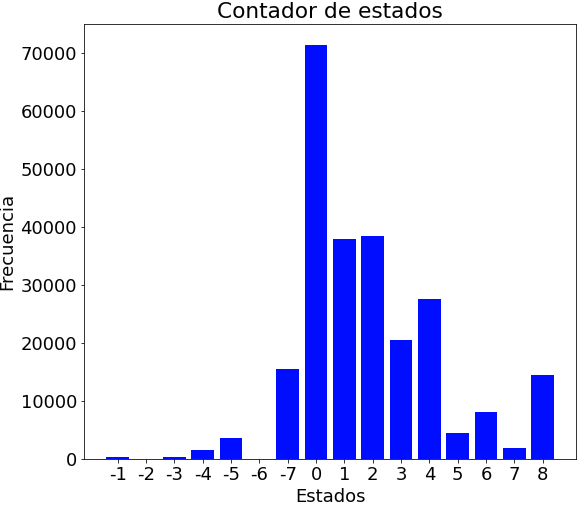
\includegraphics[width=0.6\columnwidth]{./figures/chapter_5/simple_circuit_simple_1.png}
    \caption{Análisis del número de estados de un entrenamiento en el <<Circuito Simple>>, con un nivel de percepción y un conjunto simple de acciones.}\label{fig:entrenamiento-contador-1}
\end{figure}

Dado que todos los entrenamientos tienen la misma duración, (2 horas), en el eje de abscisas puede verse en la Figura \ref{fig:entrenamiento-recompensa-1} que 2 de los 3 ensayos convergen muy rápidamente (gráficas verde y amarilla), en apenas $10$ épocas y acumulando mucha recompensa, esto es, pasa más tiempo en regiones donde la recompensa retorna los valores más altos (el centro de la línea). El último de ellos (gráfica azul) no consigue una secuencia que le permita converger tan rápidamente.\\

Se contabiliza una vuelta completa al <<Circuito Simple>> cuando se superan un número de pasos consecutivos sin reiniciar el entorno. Para el caso del <<Circuito Simple>> este valor es de $4000$ y está marcado en la gráfica de la Figura \ref{fig:entrenamiento-pasos-1} con una línea horizontal roja.\\

\begin{figure}[ht!]
    \begin{center}
        \subfloat[Recompensa acumulada por episodio.]{\label{fig:entrenamiento-recompensa-1}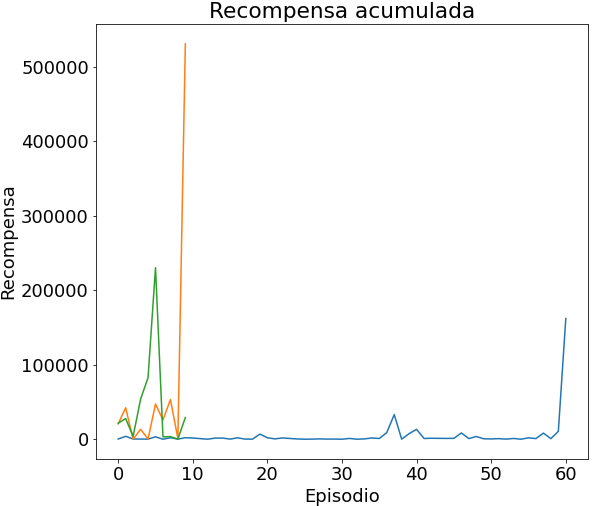
\includegraphics[width=.49\linewidth]{figures/chapter_5/simple_circuit_simple_2.png}}
        \hspace{0.1cm}
        \subfloat[Pasos por episodio.]{\label{fig:entrenamiento-pasos-1}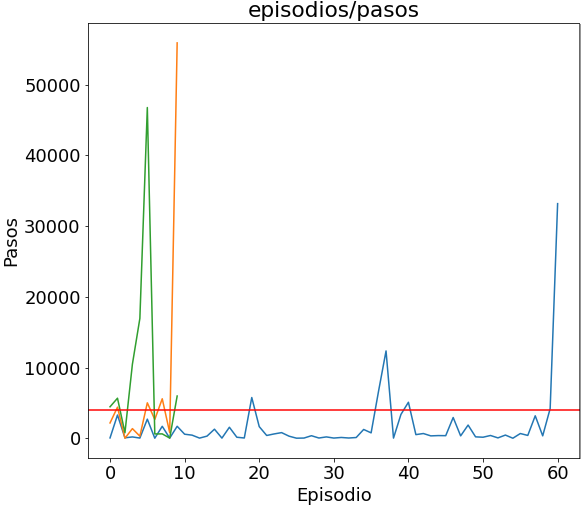
\includegraphics[width=.49\linewidth]{figures/chapter_5/simple_circuit_simple_3.png}}
    \end{center}
  \centering
  \captionsetup{justification=centering,margin=2cm}
  \caption{Análisis de un entrenamiento en el circuito simple, con un único nivel de percepción y un conjunto simple de acciones.}
  \label{fig:entrenamiento-1}
\end{figure}

La representación de estas mismas gráficas en valores numéricos puede verse en la Tabla \ref{tab:tabla-entrenamiento-1}.

\begin{table}[ht!]
\centering

\begin{tabular}{|
>{\columncolor[HTML]{EFEFEF}}l |c|c|c|}
\hline
\multicolumn{4}{|c|}{\cellcolor[HTML]{EFEFEF}\textbf{Circuito Simple}}                                                   \\ \hline
\textbf{Entrenamiento}                  & \cellcolor[HTML]{3685BB}\textbf{1} & \cellcolor[HTML]{FF8215}\textbf{2} & \cellcolor[HTML]{2CA02C}\textbf{3} \\ \hline
\textbf{Vuelta completada}         & Sí                                 & Sí                                 & Sí                                 \\ \hline
\textbf{Tiempo hasta completar}    & 20:06 min                          & 6:53 min                           & 4:26 min                           \\ \hline
\textbf{Épocas hasta completar}    & 20                                 & 2                                  & 1                                  \\ \hline
\textbf{Valor de $\epsilon$ final} & 0.8                                & 0.84                               & 0.85                               \\ \hline
\textbf{Tamaño de la Tabla-Q}      & 40                                 & 23                                 & 22                                 \\ \hline
\textbf{Total de épocas}           & 61                                 & 10                                 & 10                                 \\ \hline
\end{tabular}
\caption{Tabla resumen del conjunto de entrenamiento en el circuito <<Circuito Simple>> con 1 nivel de percepción y el conjunto de acciones simple.}
\label{tab:tabla-entrenamiento-1}
\end{table}

\newpage
Un ejemplo con otra configuración de parámetros puede verse en las Figuras \ref{fig:entrenamiento-2} y \ref{fig:entrenamiento-2-2}. En este ejemplo el circuito de entrenamiento es Nürburgring con un conjunto de acciones medio (5 acciones) y 2 puntos de percepción simplificada.\\

Puede verse que el conjunto de estados para este ensayo (figura \ref{fig:entrenamiento-2}) es más variado comparado con el anterior. Se distribuyen los valores entre más estados enriqueciendo la Tabla-Q. El estado más frecuente es el $(-2, -4)$ con un total de $33065$ veces.\\

\begin{figure}[!ht]
    \centering 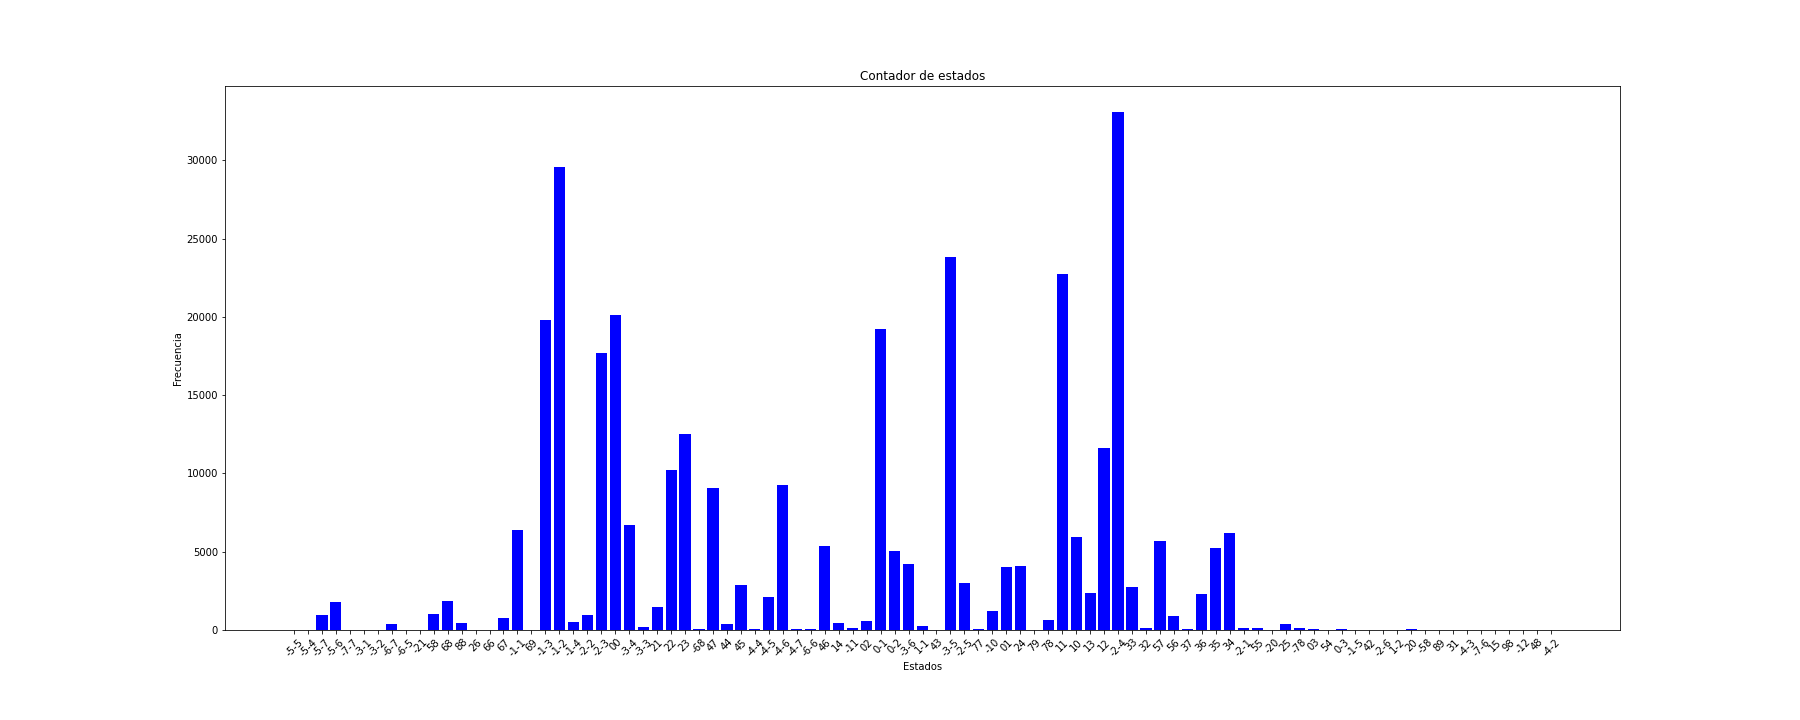
\includegraphics[width=1\columnwidth]{./figures/chapter_5/nurburgring_medium_1.png}
    \caption{Análisis del número de estados de un entrenamiento en el circuito de Nürburgring, con dos niveles de percepción y un conjunto medio de acciones.}\label{fig:entrenamiento-2}
\end{figure}

En cuanto a la recompensa acumulada durante el entrenamiento (figura \ref{fig:entrenamiento-recompensa-2}) pueden verse 3 modas que se replican en el número de pasos donde, con un valor aproximado a $4000$ pasos se considera una vuelta al circuito (marcado con una línea horizontal roja en la figura \ref{fig:entrenamiento-pasos-2}). Las tres modas superan este valor por lo que se concluye que hubo convergencia en el entrenamiento para esta configuración.

\begin{figure}[ht!]
    \begin{center}
        \subfloat[Recompensa acumulada por episodio.]{\label{fig:entrenamiento-recompensa-2}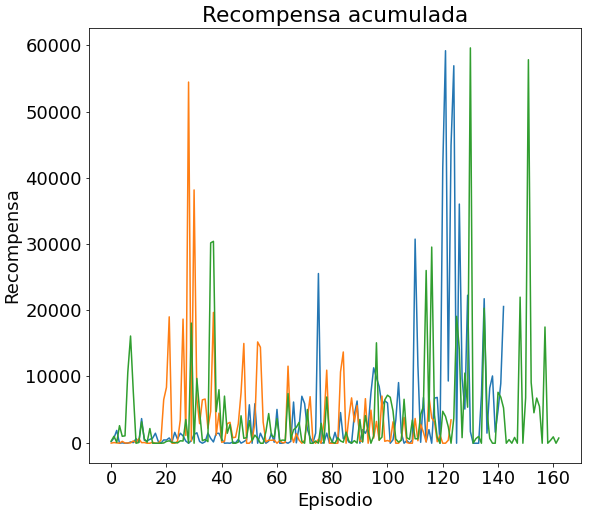
\includegraphics[width=.49\linewidth]{figures/chapter_5/nurburgring_medium_2.png}}
        \hspace{0.1cm}
        \subfloat[Pasos por episodio.]{\label{fig:entrenamiento-pasos-2}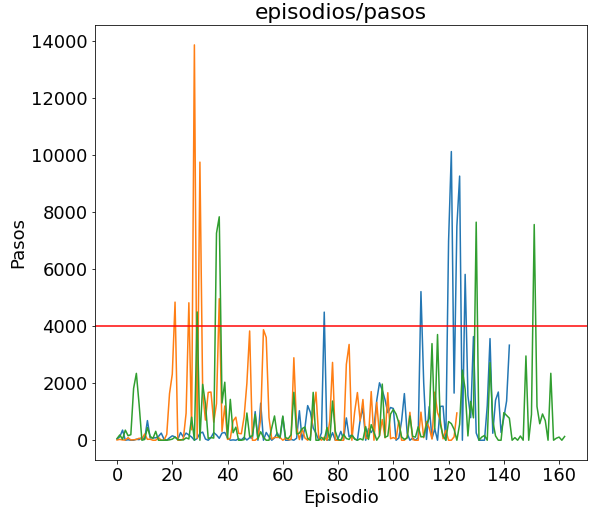
\includegraphics[width=.49\linewidth]{figures/chapter_5/nurburgring_medium_3.png}}
    \end{center}
  \centering
  \captionsetup{justification=centering,margin=2cm}
  \caption{Gráficas del estado de la recompensa y pasos dados por cada episodio.}
  \label{fig:entrenamiento-2-2}
\end{figure}

Los valores numéricos correspondientes a las gráficas pueden verse en la Tabla \ref{tab:tabla-entrenamiento-2} para cada uno de los entrenamientos.

\begin{table}[ht!]
\centering
\begin{tabular}{|
>{\columncolor[HTML]{EFEFEF}}l |c|c|c|}
\hline
\multicolumn{4}{|c|}{\cellcolor[HTML]{EFEFEF}\textbf{Nürburgring}}                                                                                \\ \hline
\textbf{Entrenamiento}                  & \cellcolor[HTML]{3685BB}\textbf{1} & \cellcolor[HTML]{FF8215}\textbf{2} & \cellcolor[HTML]{2CA02C}\textbf{3} \\ \hline
\textbf{Vuelta completada}         & Sí                                 & Sí                                 & Sí                                 \\ \hline
\textbf{Tiempo hasta completar}    & 19.32 min                          & 9:11 min                           & 13:12 min                          \\ \hline
\textbf{Épocas hasta completar}    & 75                                 & 21                                 & 29                                 \\ \hline
\textbf{Valor de $\epsilon$ final} & 0.72                               & 0.75                               & 0.72                               \\ \hline
\textbf{Tamaño de la Tabla-Q}      & 147                                & 140                                & 115                                \\ \hline
\textbf{Total de épocas}           & 143                                & 124                                & 163                                \\ \hline
\end{tabular}
\caption{Tabla resumen del entrenamiento en el circuito de Nürburgring con 2 niveles de percepción y el conjunto de acciones medio.}
\label{tab:tabla-entrenamiento-2}
\end{table}

\newpage
Pueden verse las gráficas y tablas con todas las configuraciones probadas en el Anexo \ref{anexos}, sección \ref{anexo-resultados-entrenamientos}.


%%%%%%%%%%%%%%%%%%%%%%%%%%%%%%%%%%%%%%%%%%%%%%%%%%%%%%%%%%%%%%%%%%%%%%%%%%%%%%%%%%%%%%%%%%%%%%%%%%%%%%%%%%%%%%%%
\section{Métricas de calidad de la conducción autónoma conseguida}

Una vez finalizada cada combinación de entrenamientos se ejecuta el cerebro aprendido por refuerzo para su validación. Únicamente tomará de la Tabla-Q los pares de (\textit{estado, acción}) con la mayor recompensa para cada estado. Esta acción da los valores que se envían de velocidad lineal y de velocidad angular a los motores del Fórmula-1. Este nuevo cerebro aprendido tiene 3 oportunidades para resolver una vuelta en a los circuitos de evaluación.\\

Las métricas por las que se mide la calidad de la conducción autónoma lograda con cada cerebro aprendido son:\\

\begin{itemize}
    \item Tiempo por vuelta.
    \item Porcentaje del circuito completado.\\
\end{itemize}

La métrica que evalúa la calidad del algoritmo entrenado es el `Tiempo por vuelta' para modelos que completan el circuito y la métrica `Porcentaje de circuito completado' está más enfocada a la combinación de parámetros que no consigue completar la vuelta. Si una ejecución del modelo entrenado consigue completar una vuelta en un circuito de evaluación (los dos restantes de los tres creados), se considera que la aproximación de aprendizaje por refuerzo es factible y soluciona el problema para esa configuración de parámetros. \\

Para medir el tiempo que tarda en completar la vuelta se ha diseñado un sistema automático que registra la salida y llegada a la meta y detiene el programa, mostrando el tiempo que ha tardado en resolverlo y cuántos intentos ha necesitado. Para localizar al Fórmula-1 en el circuito se utiliza la librería de Gazebo \texttt{GetModelStates}\footnote{\url{http://docs.ros.org/jade/api/gazebo_msgs/html/msg/ModelState.html}} que retorna la posición del robot en el mundo simulado. Por cada paso del Fórmula-1 se obtienen los valores $(x, y)$ y se comprueba que la distancia euclídea a la línea de salida (origen del mundo de Gazebo) no sea mayor que $0.5$ metros, dejando un margen por si el Fórmula-1 atraviesa la línea de meta ligeramente desplazado del centro del circuito. Puede verse en el fragmento \ref{lst:finish-line} el cálculo de la distancia del robot a la línea de meta.

\vspace{5mm}

\begin{tabular}{ht!}
\begin{lstlisting}[basicstyle=\ttfamily\scriptsize, caption={Cálculo de la distancia al origen del mundo de Gazebo.}, captionpos=b, numbers=none,label={lst:finish-line}, style=Python] 
def finish_line(self):
    x, y = self.get_position()
    current_position = np.array([x, y])

    dist = (self.start_pose - current_position) ** 2
    dist = np.sum(dist, axis=0)
    dist = np.sqrt(dist)
    
    if dist < max_distance:
        return True
    return False
\end{lstlisting}
\end{tabular}

\vspace{5mm}\textbf{}

Si se cumple esta condición, el programa termina cerrando la sesión del entorno de Gym-Gazebo.\\

En el caso de que el cerebro entrenado no consiga completar el circuito se toman los puntos de referencia distribuidos regularmente por el circuito para verificar cuántos de ellos ha alcanzado el piloto con aprendizaje por refuerzo. Si ha pasado cerca de un punto se considera que lo ha conseguido. De este modo se tiene una aproximación al porcentaje del circuito que ha logrado completar el piloto con aprendizaje por refuerzo.Puede verse en la figura \ref{fig:punto_control} un ejemplo en el <<Circuito Simple>> de los puntos de control generados por el piloto manual.

\begin{figure}[ht!]
    \centering 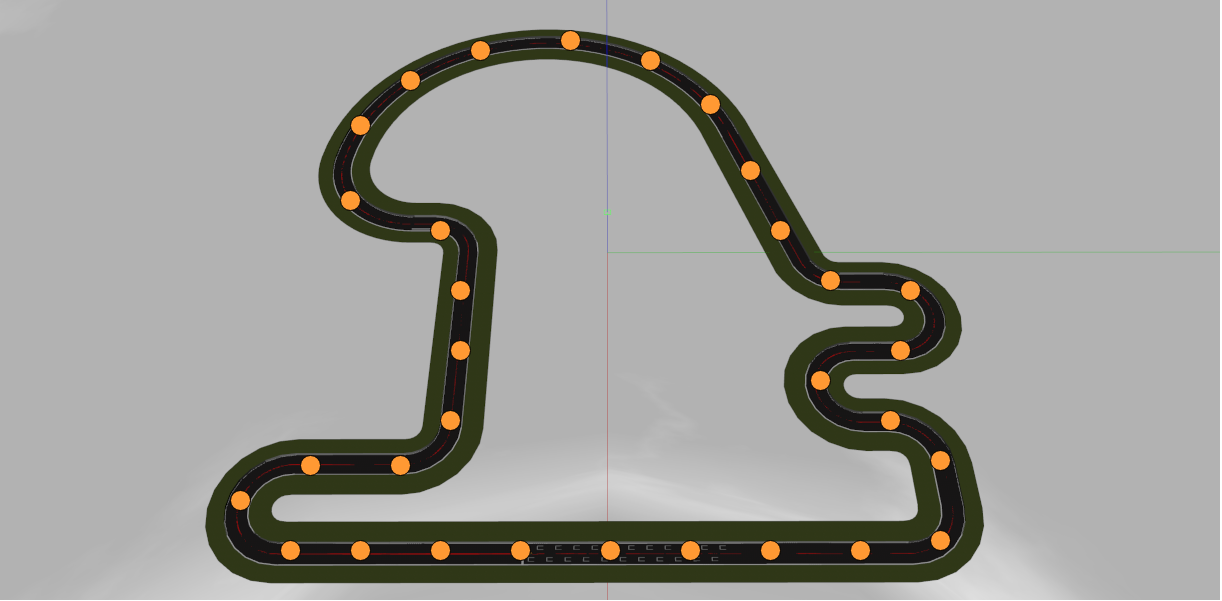
\includegraphics[width=0.5\columnwidth]{./figures/chapter_5/balizas_simple.png}
    \caption{Ejemplo de puntos de control generados por el piloto manual.}\label{fig:punto_control}
\end{figure}

Estableciendo un radio máximo de distancia de 5 metros entre el punto de referencia y el alcanzado por el entrenado se calcula el porcentaje de puntos de control que atraviesa el piloto de RL. El número de puntos generados para el <<Circuito Simple>> es de 52 y para Nürburgring de 65.


\newpage
%%%%%%%%%%%%%%%%%%%%%%%%%%%%%%%%%%%%%%%%%%%%%%%%%%%%%%%%%%%%%%%%%%%%%%%%%%%%%%%%%%%%%%%%%%%%%%%%%%%%%%%%%%%%%%%%
\section{Experimentos y ejecución típica}

Una vez ejecutados todos los cerebros aprendidos en los escenarios donde no fueron entrenados se lleva a cabo un proceso de evaluación.\\

A nivel individual se han evaluado cómo el conjunto de acciones y los niveles de percepción simplificada  afectan a los tiempos por vuelta del Fórmula-1 en cada circuito de evaluación. También se ha visto cómo en función del circuito de entrenamiento la evaluación, al ser más rica, está preparada para estados con menos frecuencia de aparición. Con el objetivo de tener una visión general de todas la evaluaciones, en la siguiente secuencia de tablas se tienen los resultados de todas las evaluaciones en los diferentes escenarios y con las diferentes configuraciones de parámetros de acciones y percepciones.\\

Las celdas marcadas en verde indican que el circuito se completó con éxito y las marcadas en naranja que solo se completó una parte y por tanto no es contabilizado el resultado como una solución válida.\\

La Tabla \ref{tab:entrenamiento-nurbur-evaluacion-simple} muestra los resultados del entrenamiento en el circuito de Nürburgring y la evaluación en el <<Circuito Simple>>.\\

\begin{table}[ht!]
\centering
\begin{tabular}{|l|c|c|c|c|c|c|c|c|c|}
\hline
\rowcolor[HTML]{EFEFEF} 
\multicolumn{10}{|c|}{\cellcolor[HTML]{EFEFEF}\textbf{Entrenamiento en Nürburgring y ejecución en <<Circuito Simple>>}}                                                                                                                                                       \\ \hline
\rowcolor[HTML]{EFEFEF} 
\textbf{Percepciones}                     & \multicolumn{9}{c|}{\cellcolor[HTML]{EFEFEF}\textbf{1 punto}}                                                                                                                                                         \\ \hline
\rowcolor[HTML]{EFEFEF} 
\textbf{Acciones}                                 & \multicolumn{3}{c|}{\cellcolor[HTML]{EFEFEF}\textbf{Simple}}             & \multicolumn{3}{c|}{\cellcolor[HTML]{EFEFEF}\textbf{Medio}}                & \multicolumn{3}{c|}{\cellcolor[HTML]{EFEFEF}\textbf{Difícil}} \\ \hline
\rowcolor[HTML]{EFEFEF} 
\textbf{Experimento}                              & \textbf{1}                    & \textbf{2} & \textbf{3}                  & \textbf{1}                    & \textbf{2}                    & \textbf{3} & \textbf{1}          & \textbf{2}         & \textbf{3}         \\ \hline
\cellcolor[HTML]{EFEFEF}\textbf{Tiempo (min)} & 3:33                          & 3:53       & \cellcolor[HTML]{32CB00}3:18                        & 3:51                          & 6:08                          & 3:33       & 5:54                & 5:51               & 4:10               \\ \hline
\cellcolor[HTML]{EFEFEF}\textbf{Intentos}         & 1                             & 1          & 1                           & 1                             & 4                             & 1          & 1                   & 2                  & 1                  \\ \hline
\rowcolor[HTML]{32CB00} 
\cellcolor[HTML]{EFEFEF}\textbf{\% de circuito}   & 100                           & 100        & \textbf{100}                & 100                           & 100                           & 100        & 100                 & 100                & 100                \\ \hline
\rowcolor[HTML]{EFEFEF} 
\textbf{Percepciones}                     & \multicolumn{9}{c|}{\cellcolor[HTML]{EFEFEF}\textbf{2 puntos}}                                                                                                                                                        \\ \hline
\cellcolor[HTML]{EFEFEF}\textbf{Tiempo (min)}          & $\infty$                        & 3:43       & 3:55                        & $\infty$                        & $\infty$                        & 5:30       & 5:45                & 5:03               & 4:32               \\ \hline
\cellcolor[HTML]{EFEFEF}\textbf{Intentos}                  & 3                             & 2          & 1                           & 3                             & 3                             & 1          & 1                   & 1                  & 1                  \\ \hline
\rowcolor[HTML]{32CB00} 
\cellcolor[HTML]{EFEFEF}\textbf{\% de circuito}            & \cellcolor[HTML]{FFC702}63.46 & 100        & 100                         & \cellcolor[HTML]{FFC702}94.23 & \cellcolor[HTML]{FFC702}34.62 & 100        & 100                 & 100                & 100                \\ \hline
\rowcolor[HTML]{EFEFEF} 
\textbf{Percepciones}                              & \multicolumn{9}{c|}{\cellcolor[HTML]{EFEFEF}\textbf{3 puntos}}                                                                                                                                                        \\ \hline
\cellcolor[HTML]{EFEFEF}\textbf{Tiempo (min)} & $\infty$                        & $\infty$     & 3.58                        & $\infty$                        & $\infty$                        & $\infty$     & $\infty$              & $\infty$             & $\infty$             \\ \hline
\cellcolor[HTML]{EFEFEF}\textbf{Intentos}         & 3                             & 3          & 3                           & 3                             & 3                             & 3          & 3                   & 3                  & 3                  \\ \hline
\rowcolor[HTML]{FFC702} 
\cellcolor[HTML]{EFEFEF}\textbf{\% de circuito}   & 17.31                         & 95.8876.92 & \cellcolor[HTML]{32CB00}100 & 34.62                         & 75                            & 78.85      & 11.54               & 19.23              & 21.15              \\ \hline
\end{tabular}
\caption{Resultados del entrenamiento en Nürburgring y la evaluación en el <<Circuito Simple>>.}
\label{tab:entrenamiento-nurbur-evaluacion-simple}
\end{table}


La Tabla \ref{tab:entrenamiento-nurbur-evaluacion-montreal} muestra los resultados del entrenamiento en el circuito de Nürburgring y la evaluación en el Montreal.

\newpage


\begin{table}[ht!]
\centering
\begin{tabular}{|l|c|c|c|c|c|c|c|c|c|}
\hline
\rowcolor[HTML]{EFEFEF} 
\multicolumn{10}{|c|}{\cellcolor[HTML]{EFEFEF}\textbf{Entrenamiento en Nürburgring y ejecución en Montreal}}                                                                                                                                                            \\ \hline
\rowcolor[HTML]{EFEFEF} 
\textbf{Percepciones}                           & \multicolumn{9}{c|}{\cellcolor[HTML]{EFEFEF}\textbf{1 punto}}                                                                                                                                                         \\ \hline
\rowcolor[HTML]{EFEFEF} 
\textbf{Acciones}                               & \multicolumn{3}{c|}{\cellcolor[HTML]{EFEFEF}\textbf{Simple}} & \multicolumn{3}{c|}{\cellcolor[HTML]{EFEFEF}\textbf{Medio}}               & \multicolumn{3}{c|}{\cellcolor[HTML]{EFEFEF}\textbf{Difícil}}              \\ \hline
\rowcolor[HTML]{EFEFEF} 
\textbf{Experimento}                            & \textbf{1}                      & \textbf{2}   & \textbf{3}  & \textbf{1}                    & \textbf{2}                   & \textbf{3} & \textbf{1}                    & \textbf{2}                    & \textbf{3} \\ \hline
\rowcolor[HTML]{FFFFFF} 
\cellcolor[HTML]{EFEFEF}\textbf{Tiempo (min)}   & 11:38                           & 11:55        & \cellcolor[HTML]{32CB00}10:54       & 12:25                         & $\infty$                      & 11:32      & 20:03                         & $\infty$                       & 14:03      \\ \hline
\rowcolor[HTML]{FFFFFF} 
\cellcolor[HTML]{EFEFEF}\textbf{Intentos}       & 1                               & 1            & 1           & 1                             & 3                            & 1          & 1                             & 3                             & 1          \\ \hline
\rowcolor[HTML]{32CB00} 
\cellcolor[HTML]{EFEFEF}\textbf{\% de circuito} & 100                             & 100          & 100         & 100                           & \cellcolor[HTML]{FFC702}7.06 & 100        & 100                           & \cellcolor[HTML]{FFC702}11.76 & 100        \\ \hline
\rowcolor[HTML]{EFEFEF} 
\textbf{Percepciones}                           & \multicolumn{9}{c|}{\cellcolor[HTML]{EFEFEF}\textbf{2 puntos}}                                                                                                                                                        \\ \hline
\rowcolor[HTML]{FFFFFF} 
\cellcolor[HTML]{EFEFEF}\textbf{Tiempo (min)}            & $\infty$                         & 19:05        & 13:30       & $\infty$                       & 13:38                        & 18:33      & $\infty$                       & 15:35                         & 13:50      \\ \hline
\rowcolor[HTML]{FFFFFF} 
\cellcolor[HTML]{EFEFEF}\textbf{Intentos}                & 3                               & 3            & 2           & 3                             & 3                            & 2          & 3                             & 1                             & 1          \\ \hline
\rowcolor[HTML]{32CB00} 
\cellcolor[HTML]{EFEFEF}\textbf{\% de circuito}          & \cellcolor[HTML]{FFC702}47.06   & 100          & 100         & \cellcolor[HTML]{FFC702}12.35 & 100                          & 100        & \cellcolor[HTML]{FFC702}41.76 & 100                           & 100        \\ \hline
\rowcolor[HTML]{EFEFEF} 
\textbf{Percepciones}                                    & \multicolumn{9}{c|}{\cellcolor[HTML]{EFEFEF}\textbf{3 puntos}}                                                                                                                                                        \\ \hline
\cellcolor[HTML]{EFEFEF}\textbf{Tiempo (min)}   & $\infty$                         & $\infty$      & $\infty$     & $\infty$                       & $\infty$                      & $\infty$    & $\infty$                       & $\infty$                       & $\infty$    \\ \hline
\cellcolor[HTML]{EFEFEF}\textbf{Intentos}       & 3                               & 3            & 3           & 3                             & 3                            & 3          & 3                             & 3                             & 3          \\ \hline
\rowcolor[HTML]{FFC702} 
\cellcolor[HTML]{EFEFEF}\textbf{\% de circuito} & 8.24                            & 95.88        & 1.65        & 6.47                          & 1.65                         & 5.88       & 1.18                          & 4.71                          & 1.18       \\ \hline
\end{tabular}
\caption{Resultados del entrenamiento en Nürburgring y la evaluación en el Montreal.}
\label{tab:entrenamiento-nurbur-evaluacion-montreal}
\end{table}


La Tabla \ref{tab:entrenamiento-simple-evaluacion-nurbur} muestra los resultados del entrenamiento en el <<Circuito Simple>> y la evaluación en el Nürburgring.


\begin{table}[ht!]
\centering
\begin{tabular}{|l|c|c|c|c|c|c|c|c|c|}
\hline
\rowcolor[HTML]{EFEFEF} 
\multicolumn{10}{|c|}{\cellcolor[HTML]{EFEFEF}\textbf{Entrenamiento en Circuito Simple y ejecución en Nürburgring}}                                                                                                                                                               \\ \hline
\rowcolor[HTML]{EFEFEF} 
\textbf{Percepciones}                           & \multicolumn{9}{c|}{\cellcolor[HTML]{EFEFEF}\textbf{1 punto}}                                                                                                                                                            \\ \hline
\rowcolor[HTML]{EFEFEF} 
\textbf{Acciones}                               & \multicolumn{3}{c|}{\cellcolor[HTML]{EFEFEF}\textbf{Simple}} & \multicolumn{3}{c|}{\cellcolor[HTML]{EFEFEF}\textbf{Medio}} & \multicolumn{3}{c|}{\cellcolor[HTML]{EFEFEF}\textbf{Difícil}}                               \\ \hline
\rowcolor[HTML]{EFEFEF} 
\textbf{Experimento}                            & \textbf{1}   & \textbf{2}   & \textbf{3}                     & \textbf{1}   & \textbf{2}   & \textbf{3}                    & \textbf{1}                    & \textbf{2}                  & \textbf{3}                    \\ \hline
\rowcolor[HTML]{FFFFFF} 
\cellcolor[HTML]{EFEFEF}\textbf{Tiempo (min)}   & 4:22         & \cellcolor[HTML]{32CB00}4:13         & $\infty$                       & 8:02         & 4:54         & 5:45                          & $\infty$                      & 5:24                        & $\infty$                      \\ \hline
\rowcolor[HTML]{FFFFFF} 
\cellcolor[HTML]{EFEFEF}\textbf{Intentos}       & 1            & 1            & 3                              & 1            & 1            & 2                             & 3                             & 1                           & 3                             \\ \hline
\rowcolor[HTML]{32CB00} 
\cellcolor[HTML]{EFEFEF}\textbf{\% de circuito} & 100          & 100          & \cellcolor[HTML]{FFC702}55.77  & 100          & 100          & 100                           & \cellcolor[HTML]{FFC702}55.77 & 100                         & \cellcolor[HTML]{FFC702}55.77 \\ \hline
\rowcolor[HTML]{EFEFEF} 
\textbf{Percepciones}                           & \multicolumn{9}{c|}{\cellcolor[HTML]{EFEFEF}\textbf{2 puntos}}                                                                                                                                                           \\ \hline
\rowcolor[HTML]{FFFFFF} 
\cellcolor[HTML]{EFEFEF}\textbf{Tiempo (min)}            & $\infty$     & $\infty$     & $\infty$                       & $\infty$     & $\infty$     & 5:22                          & $\infty$                      & 6:00                        & $\infty$                      \\ \hline
\rowcolor[HTML]{FFFFFF} 
\cellcolor[HTML]{EFEFEF}\textbf{Intentos}                & 3            & 3            & 3                              & 3            & 3            & 1                             & 3                             & 2                           & 3                             \\ \hline
\rowcolor[HTML]{FFC702} 
\cellcolor[HTML]{EFEFEF}\textbf{\% de circuito}          & 7.69         & 9.62         & 9.62                           & 9.62         & 11.54        & \cellcolor[HTML]{32CB00}100   & 15.38                         & \cellcolor[HTML]{32CB00}100 & 11.54                         \\ \hline
\rowcolor[HTML]{EFEFEF} 
\textbf{Percepciones}                                    & \multicolumn{9}{c|}{\cellcolor[HTML]{EFEFEF}\textbf{3 puntos}}                                                                                                                                                           \\ \hline
\rowcolor[HTML]{FFFFFF} 
\cellcolor[HTML]{EFEFEF}\textbf{Tiempo (min)}   & $\infty$     & $\infty$     & $\infty$                       & $\infty$     & $\infty$     & $\infty$                      & $\infty$                      & $\infty$                    & $\infty$                      \\ \hline
\rowcolor[HTML]{FFFFFF} 
\cellcolor[HTML]{EFEFEF}\textbf{Intentos}       & 3            & 3            & 3                              & 3            & 3            & 3                             & 3                             & 3                           & 3                             \\ \hline
\rowcolor[HTML]{FFC702} 
\cellcolor[HTML]{EFEFEF}\textbf{\% de circuito} & 9.62         & 7.69         & 7.69                           & 7.69         & 3.85         & 7.69                          & 0                             & 0                           & 9.62                          \\ \hline
\end{tabular}
\caption{Resultados del entrenamiento en el Circuito Simple y evaluación en Nürburgring.}
\label{tab:entrenamiento-simple-evaluacion-nurbur}
\end{table}


La Tabla \ref{tab:entrenamiento-simple-evaluacion-montreal} muestra los resultados del entrenamiento en el <<Circuito Simple>> y la evaluación en el Montreal.

\newpage

\begin{table}[ht!]
\centering
\begin{tabular}{|l|c|c|c|c|c|c|c|c|c|}
\hline
\rowcolor[HTML]{EFEFEF} 
\multicolumn{10}{|c|}{\cellcolor[HTML]{EFEFEF}\textbf{Entrenamiento en Circuito Simple y ejecución en Montreal}}                                                                                                                                        \\ \hline
\rowcolor[HTML]{EFEFEF} 
\textbf{Percepciones}                           & \multicolumn{9}{c|}{\cellcolor[HTML]{EFEFEF}\textbf{1 punto}}                                                                                                                                         \\ \hline
\rowcolor[HTML]{EFEFEF} 
\textbf{Acciones}                               & \multicolumn{3}{c|}{\cellcolor[HTML]{EFEFEF}\textbf{Simple}} & \multicolumn{3}{c|}{\cellcolor[HTML]{EFEFEF}\textbf{Medio}} & \multicolumn{3}{c|}{\cellcolor[HTML]{EFEFEF}\textbf{Difícil}}            \\ \hline
\rowcolor[HTML]{EFEFEF} 
\textbf{Experimento}                            & \textbf{1}   & \textbf{2}                      & \textbf{3}  & \textbf{1}   & \textbf{2}                     & \textbf{3}  & \textbf{1}                   & \textbf{2} & \textbf{3}                   \\ \hline
\rowcolor[HTML]{FFFFFF} 
\cellcolor[HTML]{EFEFEF}\textbf{Tiempo (min)}   & 12:47        & 11:07                           & 14:28       & 20:30        & 13:17                          & 15:29       & $\infty$                     & 14:30      & $\infty$                     \\ \hline
\rowcolor[HTML]{FFFFFF} 
\cellcolor[HTML]{EFEFEF}\textbf{Intentos}       & 2            & 1                               & 3           & 1            & 1                              & 1           & 3                            & 1          & 3                            \\ \hline
\rowcolor[HTML]{32CB00} 
\cellcolor[HTML]{EFEFEF}\textbf{\% de circuito} & 100          & 100                             & 100         & 100          & 100                            & 100         & \cellcolor[HTML]{FFC702}6.47 & 100        & \cellcolor[HTML]{FFC702}7.65 \\ \hline
\rowcolor[HTML]{EFEFEF} 
\textbf{Percepciones}                           & \multicolumn{9}{c|}{\cellcolor[HTML]{EFEFEF}\textbf{2 puntos}}                                                                                                                                        \\ \hline
\rowcolor[HTML]{FFFFFF} 
\cellcolor[HTML]{EFEFEF}\textbf{Tiempo (min)}            & 11:56        & $\infty$                        & 11:06       & 15:49        & $\infty$                       & 14:16       & $\infty$                     & 15:41      & $\infty$                     \\ \hline
\rowcolor[HTML]{FFFFFF} 
\cellcolor[HTML]{EFEFEF}\textbf{Intentos}                & 1            & 3                               & 2           & 1            & 3                              & 1           & 3                            & 1          & 3                            \\ \hline
\rowcolor[HTML]{32CB00} 
\cellcolor[HTML]{EFEFEF}\textbf{\% de circuito}          & 100          & \cellcolor[HTML]{FFC702}62.35   & 100         & 100          & \cellcolor[HTML]{FFC702}10.59  & 100         & \cellcolor[HTML]{FFC702}1.18 & 100        & \cellcolor[HTML]{FFC702}6.47 \\ \hline
\rowcolor[HTML]{EFEFEF} 
\textbf{Percepciones}                                    & \multicolumn{9}{c|}{\cellcolor[HTML]{EFEFEF}\textbf{3 puntos}}                                                                                                                                        \\ \hline
\rowcolor[HTML]{FFFFFF} 
\cellcolor[HTML]{EFEFEF}\textbf{Tiempo (min)}   & $\infty$     & $\infty$                        & $\infty$    & $\infty$     & $\infty$                       & $\infty$    & $\infty$                     & $\infty$   & $\infty$                     \\ \hline
\rowcolor[HTML]{FFFFFF} 
\cellcolor[HTML]{EFEFEF}\textbf{Intentos}       & 3            & 3                               & 3           & 3            & 3                              & 3           & 3                            & 3          & 3                            \\ \hline
\rowcolor[HTML]{FFC702} 
\cellcolor[HTML]{EFEFEF}\textbf{\% de circuito} & 8.24         & 2.94                            & 6.47        & 1.76         & 1.76                           & 1.76        & 1.18                         & 1.76       & 5.88                         \\ \hline
\end{tabular}
\caption{Resultados del entrenamiento en el Circuito Simple y evaluación en Montreal.}
\label{tab:entrenamiento-simple-evaluacion-montreal}
\end{table}

En esta sección se han visto distintos experimentos individuales y posteriormente más generales para extraer conclusiones sobre todas las evaluaciones de los cerebros aprendidos por refuerzo. Existen combinaciones de parámetros que resuelven la conducción autónoma en el circuito de manera satisfactoria y próxima en términos de tiempos por vuelta a un cerebro programado explícitamente. El algoritmo Q-Learning funciona bien para este comportamiento y lo resuelve satisfactoriamente.\\

Teniendo como referencia los tiempos por vuelta en cada circuito de un Fórmula-1 ejecutado con un código programado manualmente que resuelve el circuito de manera explícita, se selecciona el cerebro con la mejor combinación de parámetros que resuelve cada uno de ellos. En la tabla \ref{tab:mejores-resultados} puede verse el mejor tiempo para cada circuito así como la diferencia con respecto al piloto de referencia.

\begin{table}[ht!]
\centering
\begin{tabular}{|
>{\columncolor[HTML]{C0C0C0}}l |c|c|c|}
\hline
\textbf{Circuito}    & \cellcolor[HTML]{C0C0C0}\textbf{Piloto manual} & \cellcolor[HTML]{C0C0C0}\textbf{Piloto aprendido por RL} & \cellcolor[HTML]{C0C0C0}\textbf{Diferencia} \\ \hline
\textbf{Simple}      & 2.35 min                                       & 3.18 min                                           & $+$43 seg                                     \\ \hline
\textbf{Nürburgring} & 3.19 min                                       & 4.13 min                                           & $+$54 seg                                     \\ \hline
\textbf{Montreal}    & 8.45 min                                       & 10.54 min                                          & $+$2.09 min                                   \\ \hline
\end{tabular}
\caption{Tabla con los mejores tiempos por vuelta.}
\label{tab:mejores-resultados}
\end{table}

Para todos los resultados de la tabla la configuración de parámetros que mejor ha resuelto el circuito ha sido la misma: conjunto de acciones simple y 1 punto de percepción simplificada.\\

En la Figura \ref{fig:circuitos-frame} puede verse una captura tomada mientras los algoritmos entrenados por aprendizaje por refuerzo ejecutan en los diferentes circuitos. Está disponible también un vídeo \footnote{\url{https://youtu.be/3jdxZTjPCss}} con la secuencia de entrenamiento y evaluación del cerebro con aprendizaje por refuerzo.

\begin{figure}[ht!]
  \begin{center}
    \subfloat[Circuito Simple.]{\label{fig:simple_frame}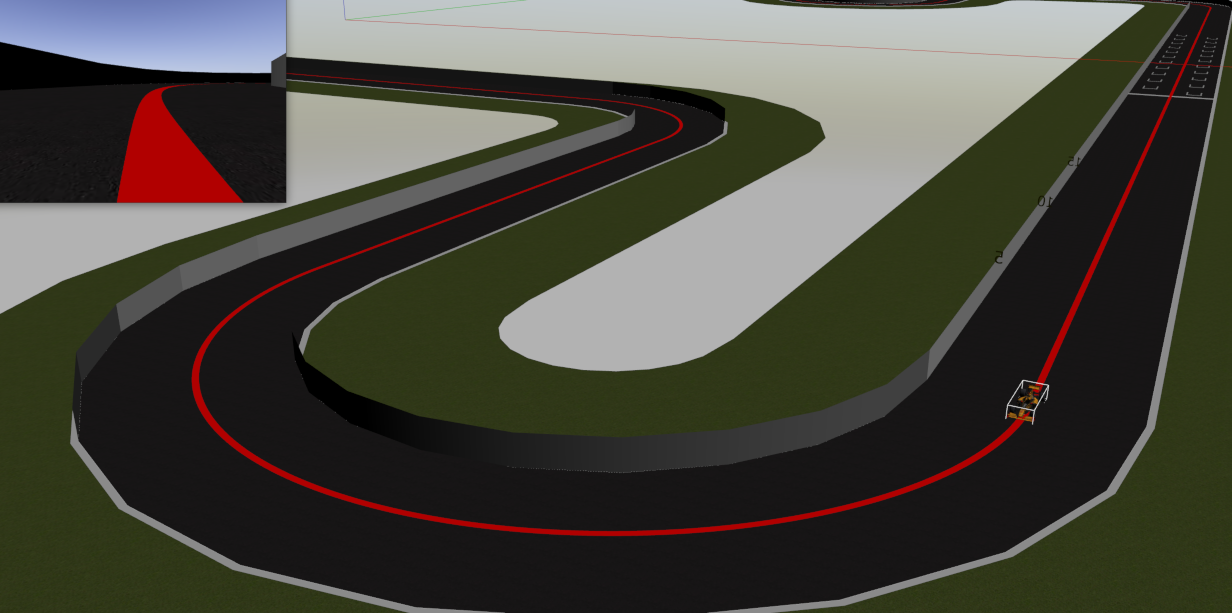
\includegraphics[width=.318\linewidth]{figures/chapter_5/simple_frame.png}}
    \hspace{0.1cm}
    \subfloat[Nürburgring.]{\label{fig:nurburgring_frame}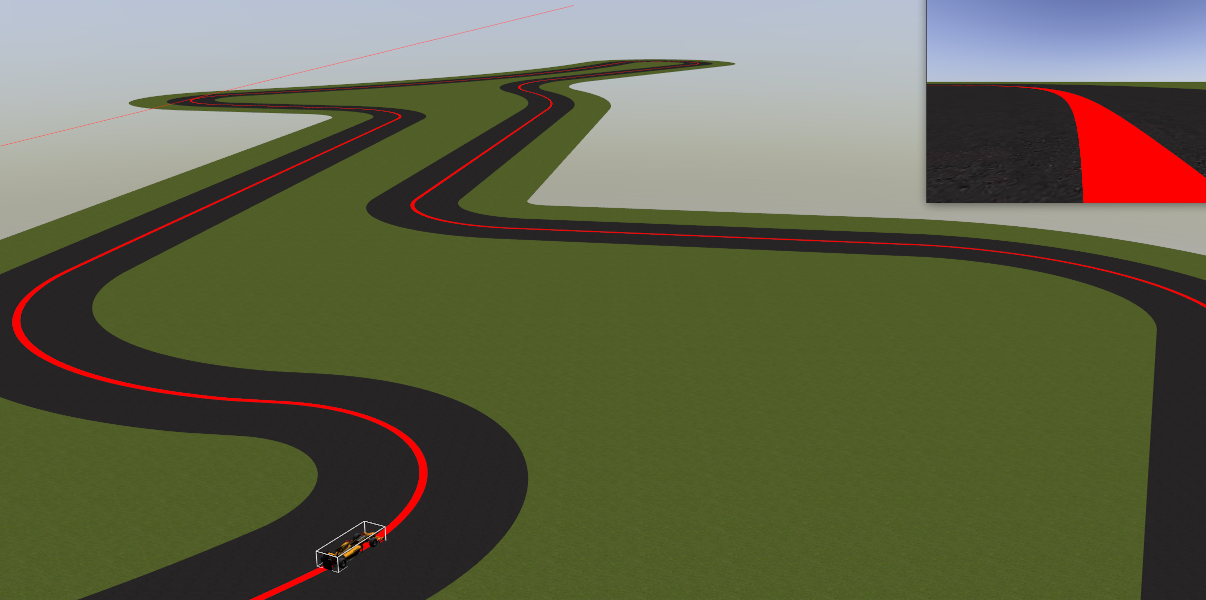
\includegraphics[width=.32\linewidth]{figures/chapter_5/nurburgring_frame.png}}
    \hspace{0.1cm}
    \subfloat[Montreal.]{\label{fig:montreal_frame}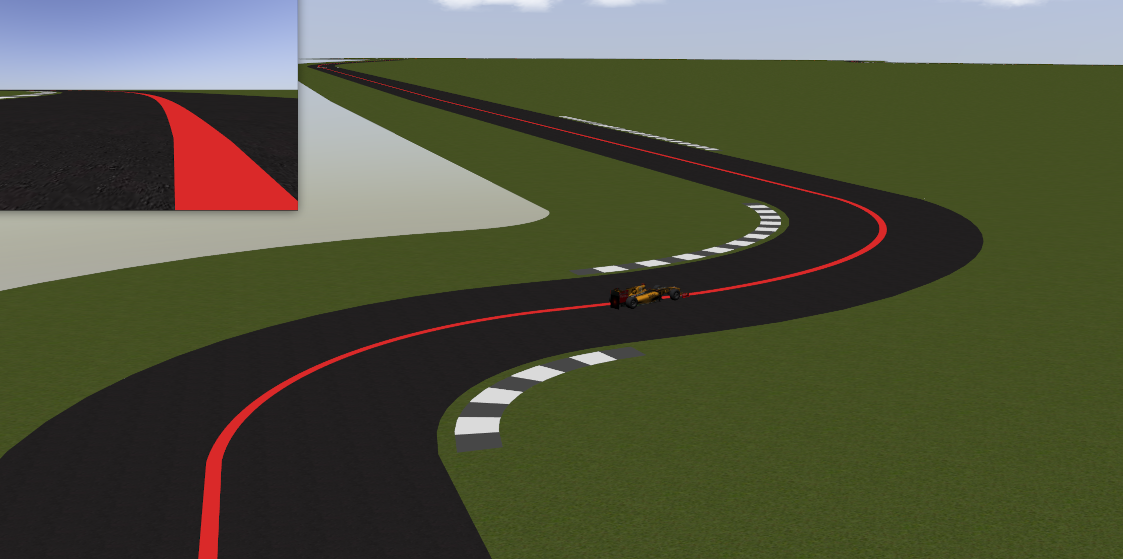
\includegraphics[width=.32\linewidth]{figures/chapter_5/montreal_frame.png}}
  \end{center}
  \centering
  \captionsetup{justification=centering,margin=2cm}
  \caption{Circuitos durante la ejecución.}
  \label{fig:circuitos-frame}
\end{figure}

El circuito de Montreal es el único en el que se prueban los entrenamientos realizados en los otros dos circuitos restantes por lo que tiene el doble de pruebas de evaluación que el resto de circuitos. El mejor tiempo por vuelta en Montreal ha sido conseguido por un modelo entrenado en Nürburgring con una diferencia de 1 minuto en promedio con respecto al mismo modelo pero entrenado en el <<Circuito Simple>>.\\

La diferencia principal de tiempos por vuelta entre el piloto manual y el aprendido por aprendizaje por refuerzo radica en dos factores:\\

\begin{itemize}
    \item En la discretización de las velocidades angulares del Fórmula-1,
    \item y en su naturaleza reactiva pura, solo tiene en cuenta información instantánea, no tiene memoria ninguna.\\
\end{itemize}

El piloto manual cuenta en su código con un mecanismo de control por realimentación proporcional, integral y derivativo (PID) que le permite corregir pequeñas desviaciones sobre la línea e incorporar en su decisión información reciente (memoria). Por ejemplo puede suavizar las respuestas si el error está reduciéndose o aumentar la respuesta si el error está creciendo. Esto se consigue porque el sistema PID puede relacionar el error actual con el error en el pasado para así ajustar más suavemente la corrección y volver a la posición central. En la figura \ref{fig:pid_control} puede verse la corrección del piloto manual ante un instante de error y como se realiza la corrección de manera suave hasta la estabilización.\\

\begin{figure}[ht!]
    \centering 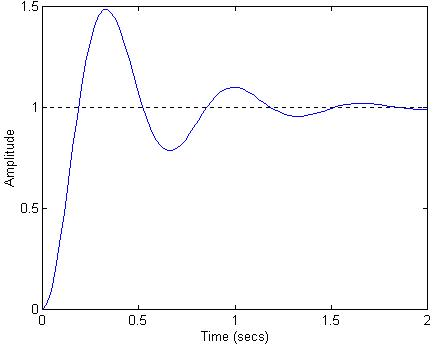
\includegraphics[width=0.5\columnwidth]{./figures/chapter_5/pid_control.jpg}
    \caption{Control proporcional, integral y derivativo del piloto manual.}\label{fig:pid_control}
\end{figure}

Por el contrario el sistema aprendido con RL es reactivo puro, rellena una tabla en la que guarda cada estado y le asocia la mejor actuación posible a la luz "únicamente" del estado actual. Sin embargo, como muestran las componentes derivativa e integral de los controladores PID, la mejor actuación posible puede depender también del estado anterior e incluso de estados previos. El sistema de RL, tal y como está construido, no lo puede tener en cuenta.\\

El comportamiento resultante del agente será más parecido a un control basado en una corrección proporcional. Puede verse en la Figura \ref{fig:p_control} un ejemplo de una secuencia de estados donde el agente de aprendizaje por refuerzo intentar corregir con las acciones de su repertorio el desvío con respecto al centro de la línea del circuito (línea roja central).\\

\begin{figure}[ht!]
    \centering 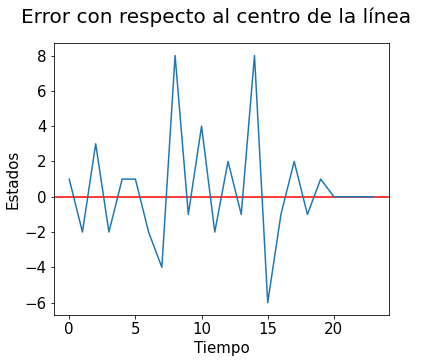
\includegraphics[width=0.5\columnwidth]{./figures/chapter_5/p_control.png}
    \caption{Control proporcional en el piloto de RL.}\label{fig:p_control}
\end{figure}

El resultado de esto son \textit{zig-zags} sobre la línea roja hasta que consigue estabilizar la dirección, en lugar de un movimiento más suave y paulatino como en el caso del PID. El tiempo de corrección hasta estabilizar el Fórmula-1 en el centro de la línea para un sistema PID es menor al conseguido con aprendizaje por refuerzo con el esquema utilizado.\\

A nivel de tiempos por vuelta se traduce en que el Fórmula-1 gobernado por un algoritmo de aprendizaje por refuerzo recorre más distancia sobre el circuito, que se traduce en mayor tiempo por vuelta.


%%%%%%%%%%%%%%%%%%%%%%%%%%%%%%%%%%%%%%%%%%%%%%%%%%%%%%%%%%%%%%%%%%%%%%%%%%%%%%%%%%%%%%%%%%%%%%%%%%%%%%%%%%%%%%%%
\section{Análisis de cardinalidad de percepciones}

Este conjunto de experimentos se centran únicamente en comparar los resultados en las configuraciones donde se modifican los niveles de percepción. Los resultados de los entrenamientos combinando los diferentes niveles muestran que el tamaño de la Tabla-Q crece al igual que la complejidad en el entrenamiento hasta completar la vuelta al circuito. El tamaño de la Tabla-Q indica lo rico que es ese conjunto de estados y que, por tanto, deberá estar más preparado ante situaciones más complejas o repentinas. A su vez el tiempo que se tarda en converger o completar el circuito es mayor y esto se traduce en que para un único nivel de percepción se necesita menor tiempo de entrenamiento y para 3 niveles se necesita, en algunos casos más tiempo de entrenamiento del que se fija en este TFM.\\

En la tabla \ref{tab:tabla-q-promedio-todos} puede verse cómo a medida que se aumentan el número de percepciones lo hace el tamaño de la Tabla-Q. Esta tabla mide un promedio de todos los entrenamientos realizados para cada una de las configuraciones de percepciones: 1, 2 y 3 puntos de percepción simplificada.

\begin{table}[ht!]
\centering
\begin{tabular}{|l|c|c|c|}
\hline
\rowcolor[HTML]{EFEFEF} 
\textbf{Puntos de percepción}                                     & \textbf{1} & \textbf{2} & \textbf{3} \\ \hline
\cellcolor[HTML]{EFEFEF}\textbf{Promedio de tamaño de la Tabla-Q} & 38         & 162        & 1062       \\ \hline
\end{tabular}
\caption{Tamaño promedio de la Tabla-Q de todos los entrenamientos}
\label{tab:tabla-q-promedio-todos}
\end{table}

El tamaño del conjunto de estados (o de la Tabla-Q) depende también del circuito donde se entrena dado que el <<Circuito Simple>> tiene un repertorio de curvas más simple que Nürburgring por lo que hay estados que solo se dan en este segundo circuito, que se traduce en que la Tabla-Q tendrá más casos. Haciendo un promedio de los tamaños de las tablas por nivel de percepción y circuito puede verse que a mismo nivel de percepción, cambiando únicamente el circuito, en ocasiones hay tablas que son más del doble de grandes. Pueden verse estos valores en la Tabla \ref{tab:media-tabla-q-percepciones}.

\begin{table}[ht!]
\centering
\begin{tabular}{|
>{\columncolor[HTML]{EFEFEF}}c |c|c|}
\hline
\multicolumn{3}{|c|}{\cellcolor[HTML]{EFEFEF}\textbf{Promedio de tamaño de las Tablas-Q}}                                        \\ \hline
\textbf{Circuito/Percepciones} & \cellcolor[HTML]{EFEFEF}\textbf{Circuito Simple} & \cellcolor[HTML]{EFEFEF}\textbf{Nürburgring} \\ \hline
\textbf{1 punto}               & 39                                               & 37                                           \\ \hline
\textbf{2 puntos}              & 143                                              & 182                                          \\ \hline
\textbf{3 puntos}              & 737                                              & 1386                                         \\ \hline
\end{tabular}
\caption{Promedio del tamaño de las Tablas-Q para distintos puntos de percepción}
\label{tab:media-tabla-q-percepciones}
\end{table}

En la Tabla \ref{tab:tiempos_percepciones} puede verse la evaluación de los tiempos por vuelta del Fórmula-1 con los distintos niveles de percepción. Para configurar esta tabla se han seleccionado los mejores tiempos para cada punto de percepción para todos los conjuntos de acciones.\\

\begin{table}[ht!]
\centering
\begin{tabular}{|l|c|c|c|c|}
\hline
\rowcolor[HTML]{EFEFEF} 
\multicolumn{5}{|c|}{\cellcolor[HTML]{EFEFEF}\textbf{Mejor tiempo / Percepciones}}                                               \\ \hline
\rowcolor[HTML]{EFEFEF} 
\textbf{Ejecutado en}                        & \textbf{Piloto Manual} & \textbf{1 punto} & \textbf{2 Puntos} & \textbf{3 Puntos} \\ \hline
\cellcolor[HTML]{EFEFEF}\textbf{Simple}      & 2.35 min               & 3.18 min         & 3.43 min          & 3.58 min          \\ \hline
\cellcolor[HTML]{EFEFEF}\textbf{Nürburgring} & 3.19 min               & 4.13 min         & 5.22 min          & -                 \\ \hline
\cellcolor[HTML]{EFEFEF}\textbf{Montreal}    & 8.45 min               & 10.54 min        & 11.06 min         & -                 \\ \hline
\end{tabular}
\caption{Mejores tiempos con diferentes puntos de percepción simplificada}
\label{tab:tiempos_percepciones}
\end{table}

La tabla de tiempos muestra que aumentando el número de percepciones se incrementan los tiempos por vuelta a diferencia de lo que puede sugerir la intuición a priori. Con el salto de un 1 punto a 2 puntos de percepción simplificada vemos que el Fórmula-1 es capaz de completar el circuito en cambio, aumentando a 3 el número de puntos perceptivos, puede verse que no se ha conseguido resolver en todos los casos.\\

Con los resultados globales en las tablas puede verse cómo según se va incrementando el número de percepciones simplificadas, en términos generales, la conducción autónoma se vuelve más compleja y no consigue resolverse.\\

Puede concluirse que \textit{el mejor conjunto de percepciones} para resolver el circuito es con \textit{una única percepción simplificada}.

%%%%%%%%%%%%%%%%%%%%%%%%%%%%%%%%%%%%%%%%%%%%%%%%%%%%%%%%%%%%%%%%%%%%%%%%%%%%%%%%%%%%%%%%%%%%%%%%%%%%%%%%%%%%%%%%
\section{Análisis de cardinalidad de acciones}

Las diferentes combinaciones de acciones permiten tener un mayor o menor número de reacciones que el agente puede emplear para resolver más o menos situaciones. Aunque inicialmente, con el juego de acciones simple (3 acciones) pueden resolverse los tres circuitos, en algunas ocasiones existe algún estado donde es necesario utilizar alguna acción extra que haga corregir la trayectoria del Fórmula-1 de manera más drástica. Por otro lado, un juego de acciones simple implica perder menos velocidad y completar la vuelta en menos tiempo. Con el conjunto de estados difícil (7 acciones) el agente es más \textit{agresivo}, lo que se traduce en cambios muy bruscos de dirección y una consiguiente reducción de la velocidad de avance y mayor tiempo en completar el circuito. Esa agresividad provoca en ocasiones que corrija en exceso y requiera reiniciar el episodio.\\

Un ejemplo donde un repertorio medio o difícil de acciones permite corregir más situaciones puede verse en la secuencia de imágenes de la Figura \ref{fig:ataque-curva} donde en un momento del circuito donde hay una curva pronunciada y el Fórmula-1 comienza a corregir tarde. La trayectoria este juego de acciones más extenso permite recuperar la posición, al tener más valores de velocidad angular entre su repertorio.

\begin{figure}[ht!]
    \centering 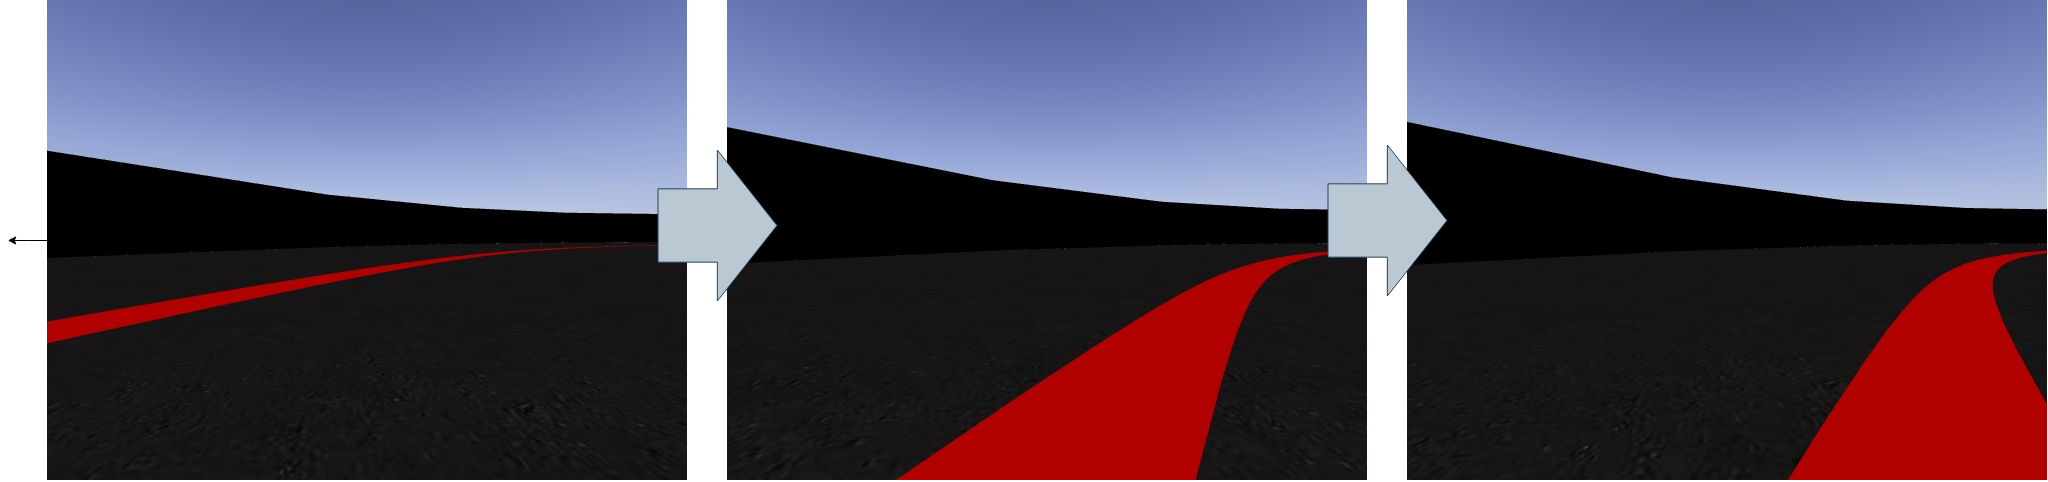
\includegraphics[width=1\columnwidth]{./figures/chapter_5/curva_pasada.png}
    \caption{Entrada en una curva por mala posición.}\label{fig:ataque-curva}
\end{figure}

Un juego de acciones simple no tendrá entre su repertorio tanta velocidad angular para poder reincorporarse a la línea y tenderá a salirse.\\

Puede verse en la tabla \ref{tab:tiempos_acciones} la relación de tiempos por vuelta para los diferentes conjuntos de acciones.

\begin{table}[ht!]
\centering
\begin{tabular}{|l|c|c|c|c|}
\hline
\rowcolor[HTML]{EFEFEF} 
\multicolumn{5}{|c|}{\cellcolor[HTML]{EFEFEF}\textbf{Mejor tiempo / Acciones}}                                              \\ \hline
\rowcolor[HTML]{EFEFEF} 
\textbf{Ejecutado en}                        & \textbf{Piloto Manual} & \textbf{Simple} & \textbf{Medio} & \textbf{Difícil} \\ \hline
\cellcolor[HTML]{EFEFEF}\textbf{Simple}      & 2.35 min               & 3.18 min        & 3.33 min       & 4,10 min         \\ \hline
\cellcolor[HTML]{EFEFEF}\textbf{Nürburgring} & 3.19 min               & 4.13 min        & 4.54 min       & 5.24 min         \\ \hline
\cellcolor[HTML]{EFEFEF}\textbf{Montreal}    & 8.45 min               & 10.54 min       & 11.06 min      & 14.03 min        \\ \hline
\end{tabular}
\caption{Mejores tiempos con diferentes conjuntos de acciones}
\label{tab:tiempos_acciones}
\end{table}

Puede concluirse que \textit{el mejor conjunto de acciones} para resolver el circuito es con \textit{un conjunto de acciones simple}.\\

Destacar que, aún perdiendo velocidad en el tiempo por vuelta, un conjunto de acciones medio otorga ese añadido necesario para que el Fórmula-1 pueda solucionar más situaciones por lo que puede ser también válido si se va a conducir autónomamente en circuito con curvas muy reviradas.\\


%%%%%%%%%%%%%%%%%%%%%%%%%%%%%%%%%%%%%%%%%%%%%%%%%%%%%%%%%%%%%%%%%%%%%%%%%%%%%%%%%%%%%%%%%%%%%%%%%%%%%%%%%%%%%%%%
\section{Influencia del circuito de entrenamiento}

Otro elemento que se tiene en cuenta en las evaluaciones experimentales es el circuito original donde se entrenaron los algoritmos de aprendizaje por refuerzo. El número de rectas, curvas a izquierdas, curvas a derechas y la complejidad de estas curvas añaden variedad que luego es utilizada en los circuitos de evaluación.\\

En la tabla \ref{tab:tiempos-circuitos} se muestra el mejor tiempo para el circuito de Montreal con los modelos entrenados en dos circuitos diferentes de entrenamiento: <<Circuito Simple>> y Nürburgring.

\begin{table}[ht!]
\centering
\begin{tabular}{|
>{\columncolor[HTML]{EFEFEF}}l |
>{\columncolor[HTML]{EFEFEF}}c |c|c|}
\hline
\multicolumn{2}{|c|}{\cellcolor[HTML]{EFEFEF}}                                             & \multicolumn{2}{c|}{\cellcolor[HTML]{EFEFEF}\textbf{Entrenado en}}                              \\ \cline{3-4} 
\multicolumn{2}{|c|}{\multirow{-2}{*}{\cellcolor[HTML]{EFEFEF}\textbf{Mejor Tiempo / Circuitos}}}   & \cellcolor[HTML]{EFEFEF}\textbf{Circuito Simple} & \cellcolor[HTML]{EFEFEF}\textbf{Nürburgring} \\ \hline
\cellcolor[HTML]{EFEFEF}                                        & \textbf{Circuito Simple} & 3:23 min                                         & 3:18 min                                     \\ \cline{2-4} 
\cellcolor[HTML]{EFEFEF}                                        & \textbf{Nürburgring}     & 4:13 min                                         & 4:12 min                                     \\ \cline{2-4} 
\multirow{-3}{*}{\cellcolor[HTML]{EFEFEF}\textbf{Ejecutado en}} & \textbf{Montreal}        & 11:06 min                                        & 10:54 min                                    \\ \hline
\end{tabular}
\caption{Entrenamiento y ejecución en diferentes circuitos.}
\label{tab:tiempos-circuitos}
\end{table}

Puede concluirse que entrenamientos en circuitos con más variedad de curvas (estados) repercute en un repertorio más robusto para afrontar cualquier circuito de evaluación. El \textit{mejor circuito} de los dos \textit{de entrenamiento} que devuelve mejores tiempos de vuelta \textit{es Nürburgring}.\\

Además, esta vista general refuerza la conclusión de que los entrenamientos en circuitos con más variedad de situaciones como Nürburgring, resuelven mejor los circuitos de evaluación. Cruzando la información entre la tabla \ref{tab:entrenamiento-simple-evaluacion-nurbur} y \ref{tab:entrenamiento-nurbur-evaluacion-simple} vemos que el segundo resuelve más casos que el primero.\\